\graphicspath{{images/}}

\section{\thesection~Methods}
\label{sec:methods}

\subsection{\thesubsection~Subsection}

\begin{Figure}
  \centering
  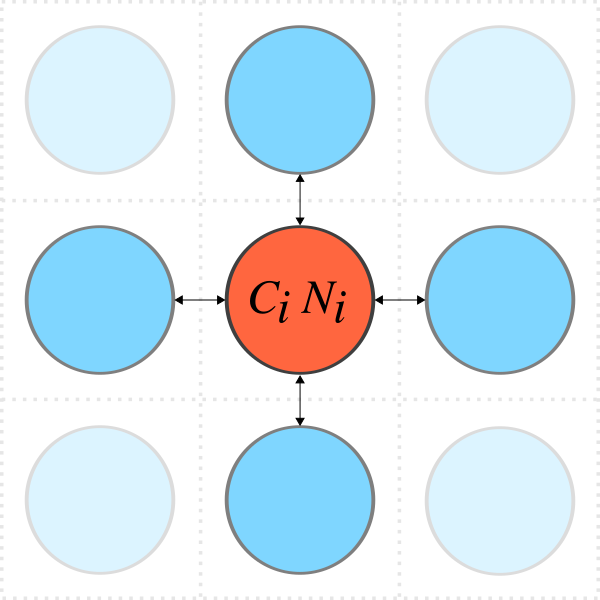
\includegraphics[width=\linewidth]{comp_model/comp_model_schematic}
  \captionof{figure}{\textbf{Schematic of the modelling approach.}
    Each circle represents a culture, indexed \(i\), growing in a grid
    on solid agar. Arrows represent the diffusion of nutrients in the
    network of cultures. \(C_{i}\) - amount of cells; \(N_{i}\) -
    amount of nutrients; darker blue circles - neighbourhood of
    culture i: \(\delta_{i}\).}
  \label{fig:comp_model_schematic}
\end{Figure}


\begin{Figure}
  \centering
  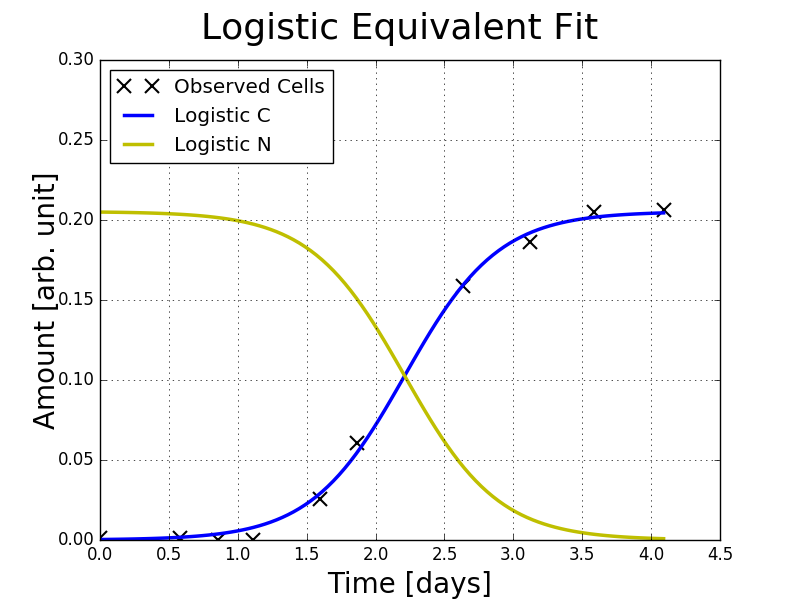
\includegraphics[width=\linewidth]{correction/log_eq_fit}
  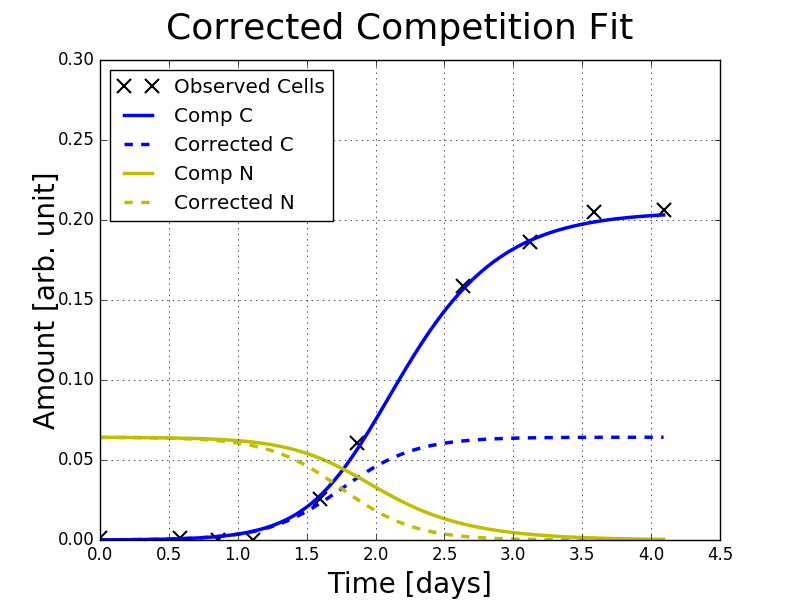
\includegraphics[width=\linewidth]{correction/comp_correction}
  \captionof{figure}{\textbf{Using the competition model to correct
      for competition.} Fits are to culture (R10, C3) of
    P15. According to the competition model, this culture reached a
    higher final cell density than its neighbours (not shown) because
    it grew faster and competed for more nutrients. The logistic
    equivalent model fit requires a higher amount of starting
    nutrients to reach the same final cell density. The correction to
    the competition model fit simulates how growth would have appeared
    without competition.}
  \label{fig:correction}
\end{Figure}

%%% Local Variables:
%%% mode: latex
%%% TeX-master: "report"
%%% End:
